\documentclass[11pt]{article}

\usepackage[a4paper, margin=1in]{geometry}

% FONTS
\usepackage[T1]{fontenc}
\usepackage{charter}  % Font face

% LAYOUT & SPACING
\usepackage{titlesec}
\usepackage{setspace}
\usepackage{fancyhdr}
\usepackage{parskip}  % no paragraph indent + space between paragraphs
\renewcommand{\baselinestretch}{1.2}  % line spacing
\setcounter{secnumdepth}{4}  % max. heading depth
\usepackage[titletoc]{appendix}

% MISC Packages
\usepackage{booktabs}  % table rules
\usepackage{tabularx}
\usepackage{hyperref}  % Links in TOC and \refs
\usepackage{apacite}
\usepackage{xcolor} % Must import BEFORE tcolorbox
\usepackage{tcolorbox}
\usepackage{tikz}
\usetikzlibrary{shapes.geometric, arrows, shadows, positioning, trees}




% HEADER & FOOTER
\pagestyle{fancy}
\fancyhf{}
\rhead{pyFin Sentiment: Financial Sentiment Analysis}
\lhead{Moritz Wilksch}
\cfoot{\thepage}

% MISC COMMANDS
\hypersetup{linktocpage, pdfborder = {0 0 0}} % Links
\hypersetup{bookmarks=true, bookmarksnumbered=true} % Links in TOC
\definecolor{up-blue}{HTML}{00305e}



% =============================================================================
\begin{document}

\tableofcontents

\newpage

% -------------- START CONTENT --------------
\section{Introduction}

The advent of social networking sites (SNS) presents the unique opportunity to tap into an enormous stream of data that users share with the world. However, most of this data comes in the form of images, videos, or text and thus is challenging to analyze. Therefore, researchers utilize automated tools to extract information from these types of media. For images, they can apply object detection to infer what kind of objects are present in a photograph. Speech detection can transcribe spoken words in videos, and named entity recognition can be utilized to recognize entities mentioned in a text. Among these technologies, sentiment analysis has been widely used by scholars and practitioners to derive actionable insights across domains. Also known as ``opinion mining'', sentiment analysis is the practice of automatically extracting sentiments or opinions from short pieces of text. Most of the time, it is measured as a real number on a continuous scale or as a categorical label like ``positive'' or ``negative''. Sentiment obtained from posts on social networks has successfully been used to detect sentiment towards political parties \shortcite{luo2022entity} or consumer products \cite{pontiki2016semeval}. If the per-document sentiment is aggregated over time, it can be used for a plethora of downstream analyses. For example, for the domain of finance, research has shown that sentiment obtained from SNS can help forecast stock market volatility \shortcite{antweiler2004all, audrino2020impact}, trading volume \shortcite{oliveira2017impact}, and even future returns \shortcite{ren2018forecasting, wilksch2022predictive}.\newline
Despite many successful applications, a problem with most sentiment analysis models is that they were designed for working with generic texts. They exploit signaling words like ``good'' or ``bad'' for determining the sentiment of a document. While it has been shown that these models perform excellently on generic social media posts \cite{al2020evaluating}, their performance on domain-specific texts is questionable. Generic sentiment models often misclassify documents containing sentiment that is easy to identify for domain experts. They lack the domain-specific connotation of terms that are only sentiment-laden in a specific domain's context. Because there are few usable domain-specific sentiment models, generic ones are still applied blindly and their output is considered ``ground truth'' for research applications studying large quantities of data. While some studies are researching alternative models for specific domains, few of them publish their models as usable artifacts to enable other researchers to benefit from more accurate sentiment assessments.

This work analyzes and proposes a solution to this issue for the domain of financial market sentiment analysis using a Design Science Research approach. Intending to build a usable model artifact that can automatically identify an author's opinion about the future of a stock's price, we collect and manually label data to compile a gold-standard dataset of finance-related tweets. We use this data to benchmark existing sentiment models trained on either generic social media data or finance-related texts. After establishing a performance benchmark of models that are popular in the literature, we design and train multiple contending sentiment models. We publish one of the proposed models as an easy-to-use python library such that future studies can utilize it for obtaining more accurate sentiment scores of finance-related social media posts. We hope this improves future research that utilizes the public social media posts of retail investors.

The remainder of this work is structured as follows. The \emph{Theoretical Background} section introduces the concepts needed for automating sentiment analysis using statistical models. It lays out how sentiment is operationalized in the literature, explains the technologies used for automating sentiment analysis, and surveys the literature on existing approaches. Finally, it highlights the research problem we aim to solve by introducing the research questions and the research paradigm we follow to answer them. The \emph{Methodology} section gives a detailed explanation of how the data used for all experiments were collected, labeled, and preprocessed. Furthermore, it lays out the experimental setup we use to train and benchmark all models. Subsequently, we present dataset statistics, an evaluation of model performance, and detailed model diagnostics in the \emph{Results} section. We highlight the issue of handling texts with no clear sentiment, provide an example use-case of how the proposed model might be used for future research, and introduce the python library that contains the final research artifact. We will discuss the emerging findings in the \emph{Discussion} and provide a final, high-level summary of the work and its findings in the \emph{Conclusion}.
\newpage
\section{Theoretical Background}



% =======================================================================
\subsection{Sentiment Analysis}  % TODO: wording

% -----------------------------------------------------------------------
\subsubsection{Operationalization of Sentiment}
\begin{itemize}[noitemsep]
	\item Definition: ``Opinion'' would be a more accurate term (Munezero, 2014)
	\item Scales: continuous $\in [-1, 1]$, discrete $\in \{pos, neg, neu\}$, 1-5 star reviews \dots
\end{itemize}

% -----------------------------------------------------------------------
\subsubsection{Sentiment in the Financial Context}

Finance-specific, alternative operationalization of sentiment:
\begin{itemize}[noitemsep]
	\item VIX
	\item Fear \& greed index, more in Aggarwal (2018)
	\item Social sentiment @IBKR?
	
\end{itemize}

% =======================================================================
\subsection{Automated Sentiment Analysis}


% -----------------------------------------------------------------------
\subsubsection{Model Perspective}
\begin{itemize}[noitemsep]
	\item Dictionaries
	\item ML
	\item DL (RNN, Transformer models)
\end{itemize}

\emph{Argument:} We can only consider models that are available as artifacts. Theoretical papers cannot be considered, as we can't reproduce their models/apply them in our experiments




% -----------------------------------------------------------------------
\subsubsection{Data Set Perspective}
Mention data-centric AI!
\begin{itemize}[noitemsep]
	\item describe different task types
	\item describe different domains + challenges (financial posts on social media)
	\begin{itemize}[noitemsep]
		\item Platforms: Twitter, StockTwits, Reddit, Crypto-specific stuff
		\item Data characteristica: Reddit posts vs. Twitter posts (compare avg. length of each?)
\end{itemize}
\end{itemize}



An example of a prompt to GPT-J \cite{gpt-j}

% =======================================================================
\subsection{Large Language Models}

% =======================================================================
\subsection{Research Gap?}
\begin{itemize}[noitemsep]
	\item performance benchmarks of LLMs (and all other models too, right?) on domain-specific texts
	\item development of a data set 	
\end{itemize}

\begin{table}[!ht]
\centering
\begin{tabular}{ccc}
	\toprule
	& \multicolumn{2}{c}{\textbf{Finance-Specific}} \\
	\cmidrule(l){2-3}
	\textbf{SNS-Specific} & Yes & No\\
	\midrule
	Yes & Sohangir (2018)$^*$ & \makecell{VADER, AFINN,\\ SentiStrength, Twitter roBERTa} \\[15pt]
	No & \makecell{Loughran\&McDonald,\\ FinBERT} & \makecell{SentiWordNet, ANEW,\\ LIWC, Harvard-IV-4, Hu \& Liu}\\
	\bottomrule
	\multicolumn{3}{l}{\footnotesize{* model artifact has not been published}}
\end{tabular}
\end{table}





% =======================================================================
\subsection{Conceptual Framework}

\begin{figure}[!ht]
	\centering
	\begin{tikzpicture}

	% --- NODES ---
	\node(m) at (-3, 0) {
		\begin{myboxprimary}{Model}{width=4.5cm}
		\begin{itemize}[noitemsep,leftmargin=*]
			\item Dictionary
			\item Machine Learning
			\item Deep Learning
		\end{itemize}	
		\end{myboxprimary}
	};
	
	\node(d) at (5, 0) {
		\begin{myboxprimary}{Dataset}{width=5cm}
		\begin{itemize}[noitemsep,leftmargin=*]
			\item SemEval2017
			\item FinancialPhrasebank
			\item Reuters TRC2
		\end{itemize}	
		\end{myboxprimary}
	};
	
	
	\node(t) at (2.5, -3.75) {
		\begin{myboxsecondary}{Task}{width=4.1cm}
		\begin{itemize}[noitemsep,leftmargin=*]
			\item 3-class polarity
			\item Continuous scale
			\item Ordinal scale
		\end{itemize}	
		\end{myboxsecondary}
	};
	
	\node(domain) at (7.5, -3.75) {
		\begin{myboxsecondary}{Domain}{width=4cm}
		\begin{itemize}[noitemsep,leftmargin=*]
			\item Twitter
			\item StockTwits
			\item News Headlines
		\end{itemize}	
		\end{myboxsecondary}
	};
	
	
	\node[draw,fit=(m)(d)(t)(domain),dashed,label=\textbf{Sentiment Analysis}]{};

	% --- ARROWS ---	
	\draw[->,line width=1pt,] (m) -- (d) node[midway,above]{based on};
	\draw[<-,line width=1pt] (t.north) -- +(0,0.4) -| (d.240) node[midway,left,yshift=0.3cm]{defines};
	
	\draw[<-,line width=1pt] (domain.north) -- +(0,0.4) -| (d.300) node[midway,right,yshift=0.3cm]{sampled from};
	
	\draw[<-,line width=1pt] (t.west) -| (m.south) node[midway,right,yshift=0.3cm]{performs};
	
	\end{tikzpicture}
\end{figure}

\emph{Research Questions}: Do LLMs perform well on domain-specific sentiment ananylsis tasks? How do they compare to smaller, machine-learning-based models as well as generic off-the-shelf models? Can simple, domain-specific models outperform LLMs/fine-tuned LLMs? Even if not, how do their memory/compute/cost footprints compare? 

Models to build:

\begin{table}[!ht]
\centering
	\begin{tabular}{ccc}
		\toprule
%		\textbf{Machine Learning} & \textbf{Deep Learning} & \textbf{Transfer Learning}\\
%		\midrule
%		Naive Bayes & Recurrent NN & BERT \\
%		Logistic Regression & Convolutional NN & DistillBERT \\
%		Random Forest & & roBERTa \\
%		LightGBM & & \\

%		\midrule
		\multicolumn{2}{c}{\textbf{Trained from Scratch}} & \textbf{Transfer Learning}\\
		\cmidrule(r){1-2} \cmidrule(l){3-3}
		\emph{Machine Learning} & \emph{Deep Learning} & \emph{Large Language Models}\\
		\midrule
		Naive Bayes & Recurrent NN & BERT \\
		Logistic Regression & Convolutional NN & DistillBERT \\
		Random Forest? & & roBERTa \\
		LightGBM? & & \\
		\bottomrule		
	\end{tabular}
	\caption{Models to build}
\end{table}









\newpage
\section{Methodology}
% =======================================================================
\subsection{Data Collection}
% -----------------------------------------------------------------------
\subsubsection{Data Sources}
English-speaking users who discuss finance and investing on online social media platforms in text form do so on three major platforms: Reddit, StockTwits, and Twitter. Reddit is a SNS on which users can create their own communities (``subreddits'') that focus on a specific topic. For example, users have created the subreddits ``Investing'' and ``StockMarket'' to discuss long-term investments and the subreddit ``WallStreetBets'' for posts about high-risk short-term gambles in the market. However, posts on Reddit tend to be much longer than posts on Twitter or StockTwits. Their length would require them to be analyzed on a paragraph- or sentence basis. Since research on SA is mostly focused on document-level analysis, we will not use Reddit posts for this work. The decision between StockTwits and Twitter is harder: posts on both platforms are similar in length and share the usage of cashtags (a ``\$'' sign followed by a ticker symbol) for identifying stocks. We decide to obtain data from Twitter rather than StockTwits for the following reasons:
\begin{enumerate}[noitemsep]
	\item The post volume on Twitter is higher than it is on StockTwits.
	\item The few data sets for SA on financial SM posts that exist use data from StockTwits, hence publishing a data set of tweets provides more value to the research community.
	\item By using Twitter data for our experiments we can answer RQ4 and compare performances between models and data sources.
\end{enumerate}

A disadvantage of the Twitter platform is that -- unlike StockTwits -- the majority of tweets are not related to finance and investing. As a remedy, we utilize cashtags for searching investment-related posts on Twitter. These tags are only used when referring to publicly traded companies as financial entities, as each cashtag contains the company's stock ticker symbol. This mostly prevents generic tweets about a company's brand or products from spilling into the collected data and allows us to focus the artifact design process on financial social media posts.

% -----------------------------------------------------------------------
\subsubsection{Sampling}
\label{section-sampling}
The first step to collecting data on Twitter is assembling a search query because the Twitter search application programming interface (API) requires users to search for specific cashtags instead of any tweet containing cashtags. To make results comparable to the previous literature we will focus on English posts only. Therefore, we use the S\&P500 index as a starting point for selecting ticker symbols to include in the search query. From there, we impose a minimum activity filter on each stock ticker: a ticker is only considered to be actively discussed on Twitter if there are more than 100 tweets per day on average mentioning it. We impose this filter because financial SA is only a valuable tool when applied to larger corpora of data. It should not be used when low post volume creates the risk of mistaking the opinion of very few people as the ``public'' sentiment. Therefore, by using an activity filter, we ensure that the tweets that are being collected are sampled from active discussions which make the training data more closely resemble the data that the SA models will be applied to at inference time. To conduct the filtering, we collect data on the number of tweets per day for every S\&P500 ticker during April of 2022. As Figure \ref{figure-tweet-activity} demonstrates, the distribution of activity is highly skewed. The top 20 tickers account for 53.7\% of all tweets about S\&P500 companies. According to the April 2022 data, 56 tickers fulfill the minimum activity constraint and account for 70.9\% of tweet volume. Out of these 56, we manually exclude 6 tickers (\texttt{AME, OGN, TEL, AMP, KEY, STX}) because while they represent corporations listed in the S\&P500 index, they are mostly used to reference cryptocurrencies on Twitter. This is problematic as the domain of cryptocurrencies is fundamentally different from the equity markets. Financial instruments like options do not exist for cryptocurrencies and they are also not affected by any kind of fundamental information. Thus, we decide to remove them from the data set and focus on publicly traded companies. This leaves 50 tickers to be included in the final Twitter API query.

\begin{figure}[!ht]
	\includegraphics[width=\textwidth]{assets/images/tweet_counts.pdf}
	\caption{Number of average tweets per day in April 2022 for the top 20 tickers}
	\label{figure-tweet-activity}
\end{figure}

The final API query is displayed in Figure \ref{figure-api-query}. The search retrieves all tweets mentioning any of the 50 tickers. Additionally, five options make the query 1) only retrieve English tweets, 2) exclude retweets because they do not contain original text, 3) exclude advertisements, 4) exclude tweets with images, and 5) exclude tweets with attached videos. We choose to exclude tweets with attached images or videos because we cannot analyze the information in the attached media. While most attachments are non-informative memes anyways, some include screenshots of stock charts or trading setups. Such images contain valuable information, but extracting it is beyond the scope of this work, which focuses on NLP.

\begin{figure}[!ht]
	\begin{tcolorbox}
	\small
	\centering
\texttt{(\$TSLA OR \$TWTR OR \$AAPL OR \$NFLX OR \$FB OR \$AMZN OR \$GM OR \$AMD OR \$NVDA OR \$MSFT OR \$DIS OR \$GOOGL OR \$F OR \$GOOG OR \$PYPL OR \$CAT OR \$T OR \$CVX OR \$BAC OR \$AAL OR \$BA OR \$PFE OR \$INTC OR \$JPM OR \$OXY OR \$ES OR \$WMT OR \$UAL OR \$DAL OR \$C OR \$KO OR \$XOM OR \$COST OR \$CCL OR \$MRNA OR \$MU OR \$GS OR \$WFC OR \$QCOM OR \$JNJ OR \$MS OR \$CRM OR \$SBUX OR \$VZ OR \$ABBV OR \$V OR \$MMM OR \$WBD OR \$NCLH OR \$PG) lang:en -is:retweet -is:nullcast -has:images -has:videos}
	\end{tcolorbox}
	\caption{Twitter API query used for data collection}
	\label{figure-api-query}
\end{figure}

Using the final search query, we collect all tweets using the Twitter API v2's endpoint \texttt{/2/tweets/search/all}. We query all tweets posted after April 1, 2021 (00:00:00 UTC) and before May 1, 2022 (00:00:00 UTC). The presented query yields $3,757,384$ raw results which are saved and will undergo further filtering and preprocessing as described in Section \ref{section-dataquality}. 
 By collecting a little more than one full year's worth of tweets we cover one full business cycle and prevent the collected data from being biased towards a small window of time, for example, earnings season. However, we have to acknowledge that market conditions and consequently Twitter discussions change over time. Therefore, the data sample from 2021/2022 might lose relevance in the long term.


% =======================================================================
\subsection{Data Labelling}

% -----------------------------------------------------------------------
\subsubsection{Data Quality Assessment}
\label{section-dataquality}
Due to resource constraints, it is infeasible to label all of the collected data. Hence, we will randomly sample $10,000$ data points which will be manually annotated. To allocate the labeling resources efficiently we clean the entire dataset before selecting the subsample to be labeled. This ensures that time invested in labeling is not wasted by removing large amounts of spam posts that could have been removed automatically.\newline
We start by removing all hyperlinks from tweets as they do not constitute natural language. This will be important for subsequent filtering operations which rely on word counts. Next, we remove all duplicates from the dataset. There are two types of duplicates we filter. First, the filter removes duplicates based on the tweet IDs in case the API returns duplicate results. Second, since a lot of the content on Twitter is generated by bots posting the same tweet multiple times, we remove all tweets that have duplicate texts which are longer than 5 words. We choose this threshold because duplicated short tweets can be legitimate messages (for example: ``bought \$TSLA''). If two tweets longer than five words are duplicated, however, they are most likely a boilerplate message posted by an automated account (for example: ``They have helped me to grow my account to almost 60K in one month, 100\% recommend joining''). Next, we filter tweets based on the number of hashtags and cashtags. A manual inspection reveals that tweets without real content often use many different hashtags or cashtags to appear in as many searches as possible. Therefore, we exclude all tweets containing five or more cashtags or eight or more hashtags. At this point, however, the data that is left still contains many spam tweets. Most of them are shorter tweets with relatively many hashtags or cashtags, but not enough to be removed by the previous filter. Hence, we impose another filter based on the ratio of cashtags to words, hashtags to words, and mentions of other users to words. We require each of these ratios to be lower or equal to $0.5$ such that a tweet must contain at least as many words as cashtags, hashtags, and mentions. Finally, the only form of unwanted tweets that still accounts for a significant amount of data is tweets about cryptocurrencies. As discussed in Section \ref{section-sampling}, we want to exclude this kind of tweet. Accordingly, we define a list of keywords that are frequently used by the cryptocurrency communities on Twitter and require there be less than or equal to two of these keywords in any tweet for it to be included in the final dataset. We allow for two keywords as we want to be conservative in removing data at this stage and stock market investors might also invest in cryptocurrencies. However, most tweets with three or more of these words are irrelevant. The keywords that were generated by iterative manual inspection of the filtering results are \emph{bitcoin, etherium, btc, eth, nft, token, wallet, web3, airdrop, wagmi, solana, opensea, cryptopunks, uniswap, lunar, hodl, binance, coinbase, cryptocom,} and \emph{doge}. Table \ref{table-samplesize-datacleaning} displays how the filtering stages reduce the sample size $n$.

\begin{table}[!ht]
	\centering
	\begin{tabular}{lcc}
		\toprule
		\textbf{Step} & \textbf{$\bm{n}$ after step} & $\bm{\Delta}$ \\
		\midrule
		data collection & $3,757,384$ & -- \\
		drop duplicates & $3,286,380$ & $-471,004$ \\
		filter number of cashtags \& hashtags & $2,797,620$ & $-488,760$ \\
		remove spam by ratios & $2,774,245$ & $-23,375$ \\
		remove cryptocurrency posts & $2,755,824$ & $-18,421$\\
		\bottomrule
	\end{tabular}
	\caption{Sample size during data cleaning stages}
	\label{table-samplesize-datacleaning}
\end{table}

From the final clean data set of $2,755,824$ tweets we sample $10,000$ for manual annotation. The sampling is conducted as a simple random sample. Alternatively to random sampling, NLP researchers can utilize active learning which promises a speed up in labeling speed. In active learning, a preliminary model is trained based on few annotated data points. Subsequently, the model can be applied to a large unlabeled corpus and return the data which are hardest to classify. These are then annotated by a human labeler. This process promises that by labeling the data that are hardest to classify, the model has more valuable information to learn from a smaller dataset which, for a data set of fixed size, should yield a better performing model. Unfortunately, the research on active learning suggests that this intuitive process only outperforms random sampling when applied to heavily unbalanced data \shortcite{miller2020active}. Because this does not apply to the data we collect we choose to stick to random sampling.


% -----------------------------------------------------------------------
\subsubsection{Task Definition}
Before labeling a subset of the collected data we need to clearly define the labeling task. This entails defining the dependent variable and laying out clear definitions for each category such that the assignment of documents to each category is as clear as possible. The dependent variable we study in this work is market sentiment. \citeA{chen2020finsome} make an important distinction between market sentiment and general author sentiment. For example, consider the sentence ``Nice, I already made a lot of money this morning and just shorted \$AAPL, this is gonna be great!''. The author's sentiment in this document is positive as they mention previous successful trades and a great future. However, the market sentiment in this sentence is negative. The author opened a short position in Apple Inc. (cashtag \$AAPL) which only yields a positive return if the stock price of Apple declines. The author, therefore, expects a decline in the market value of Apple shares which we consider a negative market sentiment. We choose to model market sentiment instead of author sentiment for the following two reasons. First, market sentiment information is more valuable for most downstream analysis tasks as it represents retail investors' anticipation of future events, not just their current general sentiment which does not need to correlate with equity markets \cite{chen2020finsome}. For example, an investor expecting a stock market crash might be happy about selling all their positions in time in which case the market sentiment (negative) and the general text sentiment (positive) might oppose one another.
 Second, the research gap outlined in Section \ref{section-research-gap} is most prevalent for the domain-specific task of market sentiment analysis as generic models like VADER \cite{hutto2014vader} or Twitter RoBERTa \cite{barbieri2020tweeteval} can be used to detect general author sentiment.
 \textcolor{red}{Add 3rd point: 3-class maps nicely to bullish/bearish/neutral}

For the data annotation task, we decide to classify documents into four categories: bullish, bearish, uncertain, and no sentiment. While this labeling scheme is different from the more common three-class approach it can account for the difference between tweets with uncertain sentiment and tweets with no sentiment. A \emph{no sentiment} category is needed because not every document contains sentimental expressions. Thus, a two-class approach that classifies documents as either positive or negative is too simplistic to be applied to real-world data. In addition to the neutral label, we add a fourth category (\emph{uncertain}) to our labeling task because for document-level analysis it is unclear to which category a tweet containing both positive \emph{and} negative sentiment belongs. The new category can capture texts like ``I like stock A but dislike stock B''. It is important to reiterate that this category does not mean that the \emph{labeler} is uncertain about what category is correct, but rather that the post contains both positive and negative aspects.
 The disadvantage of this approach is that we need a translation scheme between the labeled data obtained in this work and the more common three-class approach used by previous literature to compare model performances on different datasets. For now, we suggest that the two categories \emph{uncertain} and \emph{no sentiment} can be merged into what other research refers to as \emph{neutral}. \textcolor{red}{We will adopt this approach in the modeling phase to ensure that results obtained in this work are easily comparable to previous studies}.
 Finally, Table \ref{table-codebook} presents the detailed definitions according to which the data were labeled.




\begin{table}[!ht]
\centering
\small
\begin{tabular}{p{7.5cm}p{7.5cm}}
\toprule
\multicolumn{1}{c}{\textbf{Positive}} & \multicolumn{1}{c}{\textbf{Negative}} \\
\midrule

\begin{itemize}[noitemsep,leftmargin=*,topsep=-12pt]
	\item bought stock, holding stock, \emph{not} selling stock, want to buy stock (positive expectations)
	\item buying calls, selling puts, being long
	\item stock is a bargain, undervalued, oversold, reaching all-time high, is in an up trend
	\item positive earnings release, growing revenue, profits, or customer base, \emph{not} absolute numbers without judgement or direction
	\item price target raised
	\item made a profit, praising or giving a positive example, asking positive rhetorical question
	\item business acquisitions \& expansions

\end{itemize} & \begin{itemize}[noitemsep,leftmargin=*,topsep=-12pt]
	\item holding or selling with disappointing return
	\item buying puts, selling calls, being short
	\item not buying or selling for negative expectations
 	\item stock is overvalued, overbought, reaching a new low, is in a down trend
 	\item negative news like law suits or bad press
 	\item lowered price target
 	\item \textcolor{blue}{gloating, enjoying other's misfortune}
 	\item insulting, mocking, or giving a negative example
 	\item rhetorical questions suggesting negative sentiment 

\end{itemize}\\
\toprule
\multicolumn{1}{c}{\textbf{Uncertain}} & \multicolumn{1}{c}{\textbf{No Sentiment}} \\
\midrule

\begin{itemize}[noitemsep,leftmargin=*,topsep=-12pt]
	\item buying, selling, or not investing for uncertain expectations
	\item list pro \emph{and} con arguments for investment
	\item list positive \emph{and} negative opinions or facts in same Tweet
	\item asking for guidance because of uncertainty
	\item \emph{not:} changing one's mind, the more recent opinion counts

\end{itemize} & \begin{itemize}[noitemsep,leftmargin=*,topsep=-12pt]
	\item neutral information or news headlines
	\item absolute numbers without directional interpretation, stating non-opinionated facts that are not inherently positive or negative
	\item spam, ads, or not related to topic of investing
	\item seeking other's opinions
	\item stating an opinion which does not contain a positive or negative sentiment
\end{itemize}\\

\bottomrule
\end{tabular}
\caption{The codebook which guides the data labeling}
\label{table-codebook}
\end{table}




% =======================================================================
\subsection{Data Preprocessing}
\label{section-data-preprocessing}
% -----------------------------------------------------------------------
\subsubsection{Tokenization and Representation of Text Data}
\begin{itemize}[noitemsep]
	\item tokenization
	\item word embeddings
\end{itemize}






% =======================================================================
\subsection{Experiment Design}

%todo: this needs a section for descriptive experiments like bias check and sample tweets demo

% -----------------------------------------------------------------------
\subsubsection{Performance Evaluation}
\begin{itemize}[noitemsep]
	\item cross validation
	\item metrics
\end{itemize}


\begin{figure}[!ht]
	\centering
	\small
	\begin{tikzpicture}

	\matrix[matrix of nodes,nodes={draw,minimum width=1em,anchor=south,align=center,minimum height=1.8em,text width=5em},row sep=0.5em,column sep=-\pgflinewidth](mtx){|[fill=grey]|$t_1$ & $d_{1,1}$ & $d_{1,2}$ & $d_{1,3}$ & $d_{1,4}$ \\
	$d_{2,1}$ & |[fill=grey]|$t_2$ & $d_{2,2}$ & $d_{2,3}$ & $d_{2,4}$\\	
	$d_{3,1}$ & $d_{3,2}$ & |[fill=grey]|$t_3$ & $d_{3,3}$ & $d_{3,4}$\\		
	$d_{4,1}$ & $d_{4,2}$ & $d_{4,3}$ & |[fill=grey]|$t_4$ &  $d_{3,4}$\\		
	$d_{5,1}$ & $d_{5,2}$ & $d_{5,3}$ &  $d_{5, 4}$ & |[fill=grey]|$t_5$ \\		
	};
	
	\node[left=2em of mtx-1-1,anchor=east]{Split 1};
	\node[left=2em of mtx-2-1,anchor=east]{Split 2};	
	\node[left=2em of mtx-3-1,anchor=east]{Split 3};
	\node[left=2em of mtx-4-1,anchor=east]{Split 4};
	\node[left=2em of mtx-5-1,anchor=east]{Split 5};		

	
	\end{tikzpicture}
	\caption{Nested cross-validation split of a dataset. Grey shade represents data used for testing, white represents data used for training and validation.}
	\label{figure-cv-split}
\end{figure}


% -----------------------------------------------------------------------
\subsubsection{Selection of Models}


Models to build:

\begin{table}[!ht]
\centering
	\begin{tabular}{ccc}
		\toprule
%		\textbf{Machine Learning} & \textbf{Deep Learning} & \textbf{Transfer Learning}\\
%		\midrule
%		Naive Bayes & Recurrent NN & BERT \\
%		Logistic Regression & Convolutional NN & DistillBERT \\
%		Random Forest & & roBERTa \\
%		LightGBM & & \\

%		\midrule
		\multicolumn{2}{c}{\textbf{Trained from Scratch}} & \textbf{Transfer Learning}\\
		\cmidrule(r){1-2} \cmidrule(l){3-3}
		\emph{Machine Learning} & \emph{Deep Learning} & \emph{Large Language Models}\\
		\midrule
		Naive Bayes & Recurrent NN & BERT \\
		Logistic Regression & Convolutional NN & DistillBERT \\
		Random Forest? & & roBERTa \\
		LightGBM? & & \\
		\bottomrule		
	\end{tabular}
	\caption{Models to build}
\end{table}



\begin{itemize}[noitemsep]
	\item model types
	\item hyperparameters
\end{itemize}

% -----------------------------------------------------------------------
\subsubsection{Hyperparameters/Search Space?}


\textbf{Finally:} Show a flowchart of everything?








%\begin{figure}[!ht]
	\centering
\begin{tikzpicture}%
\node[black,minimum height=0.65cm] (h1) at (0.0,0.8) {\textbf{Words}};%
\node[black,minimum height=0.65cm] (h2) at (4.0,0.8) {\textbf{Word Embeddings}};%
\node[draw,rectangle,minimum width=1.5cm,black,opacity=0.5,align=center,minimum height=0.65cm,below=0.2cm of h1] (0) {hello};%
\node[draw,rectangle,minimum width=6cm,black,align=center,minimum height=0.65cm,below=0.2cm of h2] (vec_0) {-1.08,  -0.26,  0.11,  0.98,  0.63};%
\node[draw,rectangle,minimum width=1.5cm,black,opacity=0.5,align=center,minimum height=0.65cm,below=0.2cm of 0] (1) {this};%
\node[draw,rectangle,minimum width=6cm,black,align=center,minimum height=0.65cm,below=0.2cm of vec_0] (vec_1) {0.90,  -2.96,  0.79,  0.83,  -0.97};%
\node[draw,rectangle,minimum width=1.5cm,black,opacity=0.5,align=center,minimum height=0.65cm,below=0.2cm of 1] (2) {is};%
\node[draw,rectangle,minimum width=6cm,black,align=center,minimum height=0.65cm,below=0.2cm of vec_1] (vec_2) {0.68,  0.57,  2.48,  -0.26,  1.69};%
\node[draw,rectangle,minimum width=1.5cm,black,opacity=0.5,align=center,minimum height=0.65cm,below=0.2cm of 2] (3) {a};%
\node[draw,rectangle,minimum width=6cm,black,align=center,minimum height=0.65cm,below=0.2cm of vec_2] (vec_3) {0.42,  -2.45,  0.46,  1.93,  -0.99};%
\node[draw,rectangle,minimum width=1.5cm,black,opacity=0.5,align=center,minimum height=0.65cm,below=0.2cm of 3] (4) {good};%
\node[draw,rectangle,minimum width=6cm,black,align=center,minimum height=0.65cm,below=0.2cm of vec_3] (vec_4) {1.29,  -0.98,  0.13,  1.39,  -1.65};%
\node[draw,rectangle,minimum width=1.5cm,black,opacity=0.5,align=center,minimum height=0.65cm,below=0.2cm of 4] (5) {test};%
\node[draw,rectangle,minimum width=6cm,black,align=center,minimum height=0.65cm,below=0.2cm of vec_4] (vec_5) {-0.44,  -0.64,  -0.45,  0.05,  -1.15};%
\node[draw,red,fit=(vec_1) (vec_2),inner sep=0.1cm,line width=1pt] {};%
\end{tikzpicture}%
\caption{Word embeddings for an example sentence}
\end{figure}
\definecolor{lightgrey}{HTML}{DDDDDD}

\begin{figure}[!ht]
	\centering
	\begin{tikzpicture}
		\definecolor{grey}{HTML}{999999}
		\tikzstyle{mystyle}=[draw,grey,opacity=0,anchor=east]
		\tikzstyle{level1style}=[draw,minimum height=18pt]
		
		\node[mystyle](l1) at (-3.5, 0.5) {Word};
		\node[mystyle](l1) at (-3.5, -1) {Tokens};
		
		\draw
			node[rectangle,draw,line width=1pt,fill=lightgrey](word) at (-0.5,0.5) {university}
			node[level1style](n1) at (-2, -1) {uni}
			node[level1style](n2) at (-1, -1) {niv}		
			node[level1style](n3) at (0, -1) {...}
			node	[level1style](n4) at (1, -1) {ity};
		
		\coordinate[above=0.25cm of n1](c1);
		\coordinate[above=0.25cm of n2](c2);
		\coordinate[above=0.25cm of n3](c3);
		\coordinate[above=0.25cm of n4](c4);
		
		\draw 
			(n1.north) -- (c1) -| (word.south)
			(n2.north) -- (c2) -| (word.south)
			(n3.north) -- (c3) -| (word.south)
			(n4.north) -- (c4) -| (word.south);
		
	\end{tikzpicture}
	\caption{An example tikz figure showing a diagram}
\end{figure}
%
\begin{figure}[!ht]
	\centering
	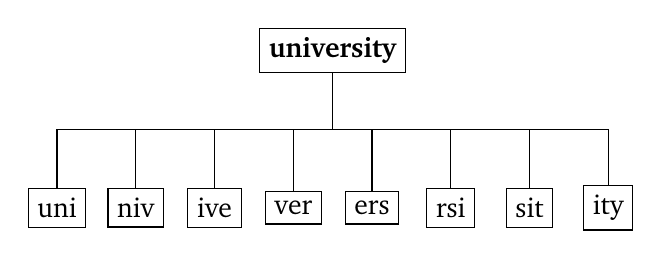
\begin{tikzpicture}
	[
		level 1/.style={level distance=2cm, sibling distance=1cm},
		edge from parent fork down
	]
		\node[draw] {\textbf {university}}
    	child {node[draw] {uni}}
	    child {node[draw] {niv}}
	    child {node[draw] {ive}}
	    child {node[draw] {ver}}
	    child {node[draw] {ers}}
	    child {node[draw] {rsi}}
	    child {node[draw] {sit}}
	    child {node[draw] {ity}};
\end{tikzpicture}
\end{figure}




\newpage

% -------------- START REFERENCES --------------
\bibliography{bibliography/refs}{}
\bibliographystyle{apacite}

% -------------- START APPENDIX --------------
\newpage % TODO: extract to file
\begin{appendices}
\section{Section Heading}
Hello Test
\end{appendices}




\end{document}